%%%%%%%%%%%%%%%%%%%%%%%%%%%%%%%%%%%%
% Slide options
%%%%%%%%%%%%%%%%%%%%%%%%%%%%%%%%%%%%

% Option 1: Slides with solutions

\documentclass[t,compress,mathserif]{beamer}
\newcommand{\soln}[1]{\textit{#1}}
\newcommand{\solnGr}[1]{#1}

% Option 2: Handouts without solutions

%\documentclass[11pt,containsverbatim,handout]{beamer}
%\usepackage{pgfpages}
%\pgfpagesuselayout{4 on 1}[letterpaper,landscape,border shrink=5mm]
%\newcommand{\soln}[1]{ }
%\newcommand{\solnGr}{ }


%%%%%%%%%%%%%%%%%%%%%%%%%%%%%%%%%%%%
% Style
%%%%%%%%%%%%%%%%%%%%%%%%%%%%%%%%%%%%

\def\chpv@path{../../Chp 5}
\def\weekv@path{../../Week5}
\input{../../lec_style.tex}


%%%%%%%%%%%%%%%%%%%%%%%%%%%%%%%%%%%%
% Preamble
%%%%%%%%%%%%%%%%%%%%%%%%%%%%%%%%%%%%

\title[Lecture 15]{MA213: Lecture 15}
\subtitle{Module 3: Foundations for inference}
\author{OpenIntro Statistics, 4th Edition}
\institute{$\:$ \\ {\footnotesize Based on slides developed by Mine \c{C}etinkaya-Rundel of OpenIntro. \\
The slides may be copied, edited, and/or shared via the \webLink{http://creativecommons.org/licenses/by-sa/3.0/us/}{CC BY-SA license.} \\
Some images may be included under fair use guidelines (educational purposes).}}
\date{}


%%%%%%%%%%%%%%%%%%%%%%%%%%%%%%%%%%%%
% Begin document
%%%%%%%%%%%%%%%%%%%%%%%%%%%%%%%%%%%%

\begin{document}


%%%%%%%%%%%%%%%%%%%%%%%%%%%%%%%%%%%%
% Title page
%%%%%%%%%%%%%%%%%%%%%%%%%%%%%%%%%%%%

{
\addtocounter{framenumber}{-1} 
{\removepagenumbers 
\usebackgroundtemplate{\includegraphics[width=\paperwidth]{../../OpenIntro_Grid_4_3-01.jpg}}
\begin{frame}

\hfill \includegraphics[width=20mm]{../../oiLogo_highres}

\titlepage

\end{frame}
}
}


%%%%%%%%%%%%%%%%%%%%%%%%%%%%%%%%%%%%
% Sections
%%%%%%%%%%%%%%%%%%%%%%%%%%%%%%%%%%%%


%%%%%%%%%%%%%%%%%%%%%%%%%%%%%%%%%%%%
% Recap/Agenda 
%%%%%%%%%%%%%%%%%%%%%%%%%%%%%%%%%%%%
% TODO better formatting
\begin{frame}
    \frametitle{Lecture 15: Agenda}
    \begin{itemize}
        \item \hl{Previously: }Probability distributions and random variables (Chapter 4)
        \item \hl{This time: }Point estimates and sampling variability (Chapter 5.1)
        \item \hl{Reading: }Chapter 5.2 for next time
        \item \hl{Deadlines/Announcements: }HW 2.3 due today, Q1 retake in discussions
    \end{itemize}
    
\end{frame}
    

%%%%%%%%%%%%%%%%%%%%%%%%%%%%%%%%%%%%

\begin{frame}
\frametitle{Poisson distribution}

The \hl{Poisson distribution} models the count of events occurring in a fixed interval of time or space, given a constant average rate and independence between events.

\begin{small}
$X \sim \text{Poisson}(\lambda) \quad
Pr(X=k) = \frac{\lambda^k e^{-\lambda}}{k!}, 
\quad k = 0, 1, 2, \ldots$
\end{small}
% \vspace{-0.5cm}
\twocol{0.4}{0.6}{
    \begin{center}
        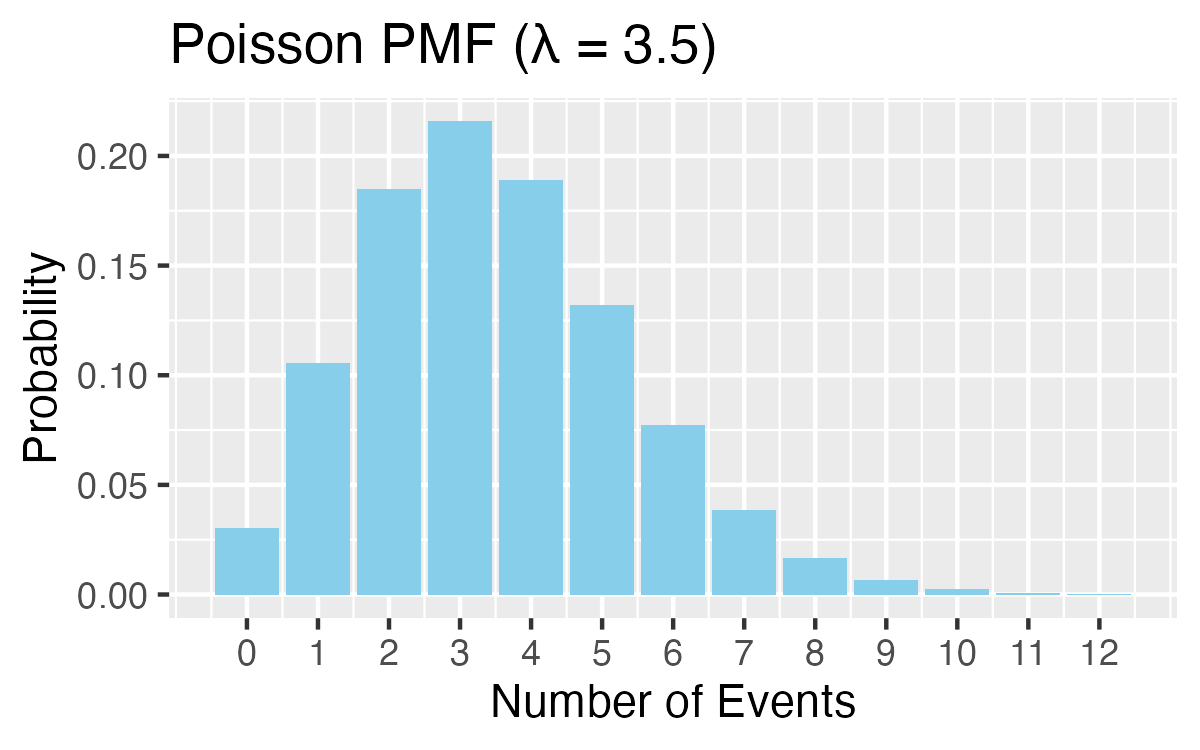
\includegraphics[height=0.25\paperheight]{\weekv@path/figures/Poisson_PMF.png}
        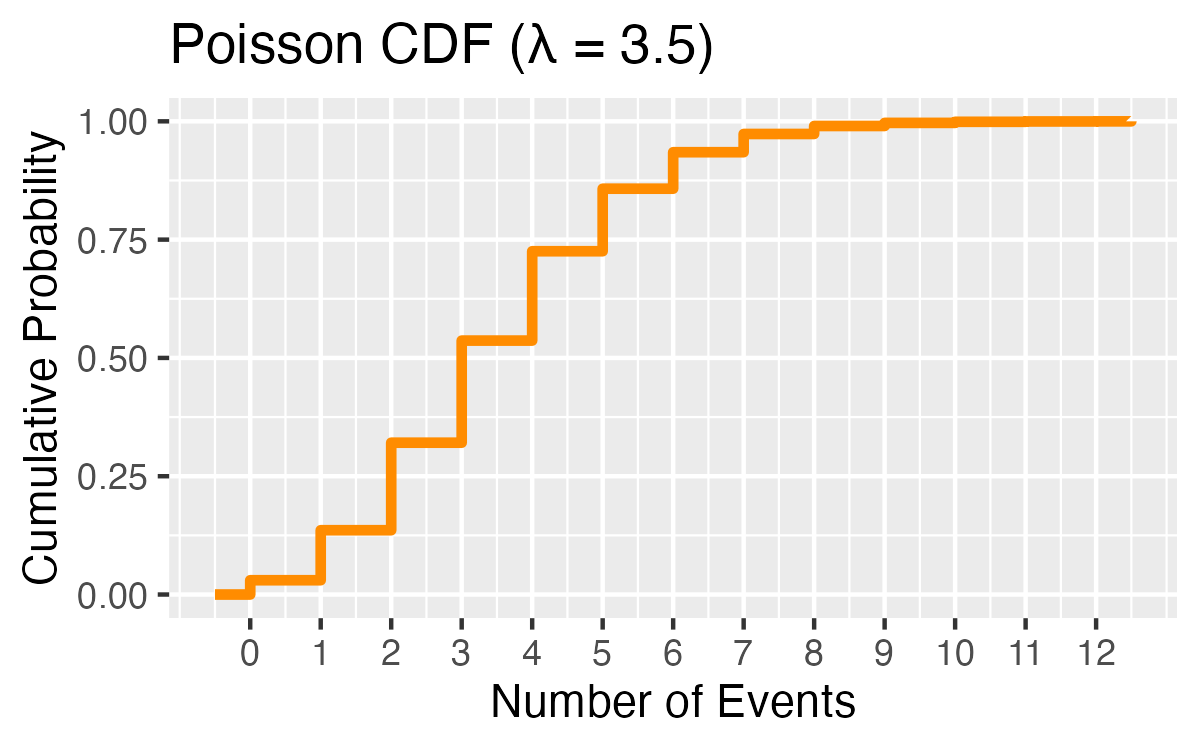
\includegraphics[height=0.25\paperheight]{\weekv@path/figures/Poisson_CDF.png}
    \end{center}
}{
    % Poisson Distribution PMF Table
    \begin{small}
    \begin{center}
    \renewcommand{\arraystretch}{1.5}
    \begin{tabular}{l | c | c }
    Event                  & $X$   & $P(X)$                        \\
    \hline
    $0$ events             & $0$   & $e^{-\lambda}$   \\
    $1$ event              & $1$   & $\frac{\lambda^1 e^{-\lambda}}{1!}$   \\
    $\vdots$               & $\vdots$ & $\vdots$                   \\
    $k$ events             & $k$   & $\frac{\lambda^k e^{-\lambda}}{k!}$   \\
    $\vdots$               & $\vdots$ & $\vdots$                   \\
    \hline
    Total                  &       & $1$                           \\
    \end{tabular}
    \end{center}
    \end{small}
}

\end{frame}

%%%%%%%%%%%%%%%%%%%%%%%%%%%%%%%%%%%%

\begin{frame}

\dq{Suppose that in a rural region of a developing country electricity power failures occur following a Poisson distribution with an average of 2 failures every week. Calculate the probability that on a given \underline{day} the electricity fails three times.}

\pause

We are given the weekly failure rate, but to answer this question we need to first calculate the average rate of failure on a given day: $\lambda_{day} = \frac{2}{7} = 0.2857$. Note that we are assuming that the probability of power failure is the same on any day of the week, i.e. we assume independence.

\pause

\begin{eqnarray*}
P(\text{3 failures on a given day}) &=& \frac{0.2857^3 \times e^{-0.2857}}{3!} \\
\pause
&=& \frac{0.2857^3 \times e^{-0.2857}}{6} \\
\pause
&=& 0.0029
\end{eqnarray*}

\end{frame}

%%%%%%%%%%%%%%%%%%%%%%%%%%%%%%%%%%%%

\section{Edfinity quiz: Modeling with the Poisson distribution}

%%%%%%%%%%%%%%%%%%%%%%%%%%%%%%%%%%%%
\begin{frame}
\frametitle{Is it Poisson?}
\begin{small}
\begin{itemize}

\item A random variable may follow a Poisson distribution if the events occur independently of each other (typically, when the population is large and the events are rare) and the rate of events is constant

\item However we can think of situations where the rate is not constant. For example, if we are interested in count of weddings over one summer, we should take into consideration that weekends are more popular for weddings.

\item In this case, a Poisson model may sometimes still be reasonable if we allow it to have a different rate for different times; we could model the rate as higher on weekends than on weekdays.

\item The idea of modeling rates for a Poisson distribution against a second variable (day of the week) forms the
foundation of some more advanced methods called \hl{generalized linear models}. There are beyond the scope of this course, but we will discuss a foundation of linear models in Chapters 7 and 8.

\end{itemize}
\end{small}

\end{frame}

%%%%%%%%%%%%%%%%%%%%%%%%%%%%

\begin{frame}
\frametitle{Comparing Binomial and Poisson Distributions}

The Poisson and Binomial distributions both count occurrences of independent events

\vspace{0.3cm}

\begin{tabular}{|p{0.45\textwidth}|p{0.45\textwidth}|}
\hline
\rowcolor{gray!20}
\textbf{Binomial $(n, p)$} & \textbf{Poisson $(\lambda)$} \\
\hline
Counting \# successes out of $n$ trials, each with probability $p$ & Counting \# events in a time (or space) interval, with rate $\lambda$ \\
\hline
Trials are independent & Events are independent \\
\hline
$Pr(X = x) = \dbinom{n}{x} p^x (1-p)^{n-x}$ \newline $x \in \{0,1,2,\ldots,n\}$ & $Pr(X = x) = \dfrac{\lambda^x e^{-\lambda}}{x!}$ \newline $x \in \{0,1,2,\ldots\}$ \\
\hline
$E[X] = np$ & $E[X] = \lambda$ \\
\hline
$Var[X] = np(1-p)$ & $Var[X] = \lambda$ \\
\hline
\end{tabular}

\small{For more detail on the relationship between the Binomial and Poisson distributions, see the slides that we didn't cover in Lecture 14 and the R demo Lecture14\_demo3.R.}

\end{frame}

%%%%%%%%%%%%%%%%%%%%%%%%%%%%

\section{Edfinity quiz: Choosing Probability Models}

%%%%%%%%%%%%%%%%%%%%%%%%%%%%%%%%%%%%

\section{Module 3: Foundations for inference}

%%%%%%%%%%%%%%%%%%%%%%%%%%%%%%%%%%%%

\begin{frame}
    \frametitle{Module 3: Foundations for inference}

    Up until now, we have talked about:
    \begin{itemize}
        \item \hl{Module 1. }Exploratory Data Analysis and Study Design
        \begin{itemize}
            \item Often we don't have access to a whole \hl{population} of interest, so we draw a random \hl{sample}
            \item A \hl{sample statistic} is a value computed from a data sample, like a sample mean
        \end{itemize}
        \pause
        \item \hl{Module 2. }Probability, Random Variables, and Distributions
        \begin{itemize}
            \item We use probability theory to model \hl{random experiments}, like drawing a random sample from a population
            \item The parameters of the models are called \hl{population parameters}
        \end{itemize}
    \end{itemize}
   
    \pause
    \begin{center}
        How can we use \hl{sample statistics} to learn about \hl{population parameters}?\\
        \hl{Module 3. }Foundations for inference
    \end{center}
\end{frame}

%%%%%%%%%%%%%%%%%%%%%%%%%%%%%%%%%%%%

\section{Point estimates and sampling variability (Ch. 5.1)}

%%%%%%%%%%%%%%%%%%%%%%%%%%%%%%%%%%%%

\begin{frame}
    \frametitle{Point estimates and error}

    \begin{itemize}

        \item We are often interested in \hl{population parameters}.
        \item Complete populations are difficult to collect data on, so we use \hl{sample statistics} as \hl{point estimates} for the unknown population parameters of interest.
        \item \hl{Error} in the estimate = difference between population parameter and sample statistic
        \item \hl{Bias} is systematic tendency to over- or under-estimate the true population parameter.
        \item \hl{Sampling error} describes how much an estimate will tend to vary from one sample to the next.
        \item Much of statistics is focused on understanding and quantifying sampling error, and \hl{sample size} is helpful for quantifying this error.

    \end{itemize}

\end{frame}

%%%%%%%%%%%%%%%%%%%%%%%%%%%%%%%%

%%%%%%%%%%%%%%%%%%%%%%%%%%%%%%%%%%%

\begin{frame}
    \frametitle{}
    
    \dq{Suppose we randomly sample 1,000 adults from each state in the US. Would you expect the sample means of their heights to be the same, somewhat different, or very different?}
    
    \pause
    
    \soln{Not the same, but only somewhat different.}
    
\end{frame}

%%%%%%%%%%%%%%%%%%%%%%%%%%%%%%%%%%%%

\subsection{Understanding the variability of a point estimate}

%%%%%%%%%%%%%%%%%%%%%%%%%%%%%%%%%%%%

\begin{frame}
    \frametitle{}
    
    \begin{center}
    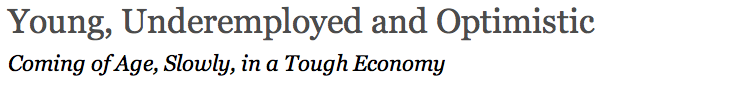
\includegraphics[width=0.95\textwidth]{\chpv@path/5-1_point_est_sampling_var/figures/pew/pew1} \\
    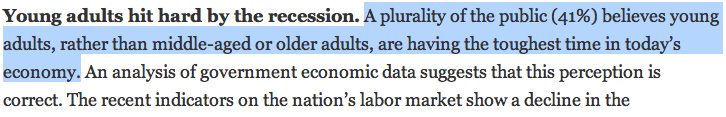
\includegraphics[width=0.95\textwidth]{\chpv@path/5-1_point_est_sampling_var/figures/pew/pew2} \\
    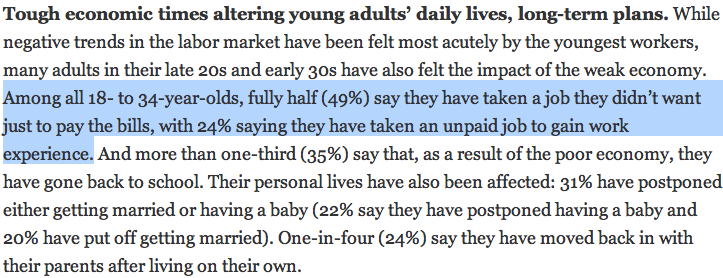
\includegraphics[width=0.95\textwidth]{\chpv@path/5-1_point_est_sampling_var/figures/pew/pew3}
    \end{center}
    
    \ct{\webURL{http://pewresearch.org/pubs/2191/young-adults-workers-labor-market-pay-careers-advancement-recession}}
    
\end{frame}

%%%%%%%%%%%%%%%%%%%%%%%%%%%%%%%%%%%%

\begin{frame}
    \frametitle{Margin of error}
    
    \begin{center}
    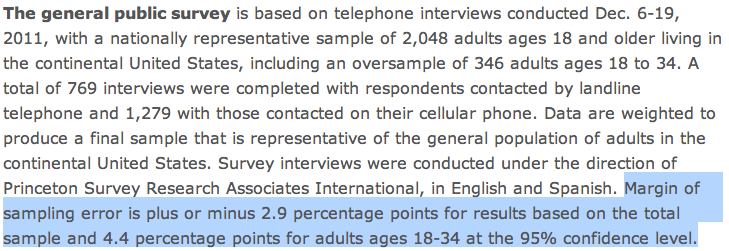
\includegraphics[width=0.95\textwidth]{\chpv@path/5-1_point_est_sampling_var/figures/pew/pew4}
    \end{center}
    
    \begin{itemize}
    
    \item 41\% $\pm$ 2.9\%: We are 95\% confident that 38.1\% to 43.9\% of the public believe young adults, rather than middle-aged or older adults, are having the toughest time in today's economy.
    
    \item 49\% $\pm$ 4.4\%: We are 95\% confident that 44.6\% to 53.4\% of 18-34 years olds have taken a job they didn't want just to pay the bills.
    
    \end{itemize}
    
\end{frame}

%%%%%%%%%%%%%%%%%%%%%%%%%%%%%%%%%%%

\begin{frame}
    \frametitle{}
    
    \dq{Suppose the proportion of American adults who support the expansion of solar energy is p = 0.88, which is our parameter of interest. Is a randomly selected American adult more or less likely to support the expansion of solar energy?}
    
    \pause
    
    \soln{More likely.}
    
\end{frame}

%%%%%%%%%%%%%%%%%%%%%%%%%%%%%%%%

\begin{frame}
    \frametitle{}
    
    \dq{Suppose that you don't have access to the population of all American adults, which is a quite likely scenario. In order to estimate the proportion of American adults who support solar power expansion, you might sample from the population and use your sample proportion as the best guess for the unknown population proportion.}
    
    \begin{itemize}
    
    \item Sample 1000 American adults from the population, and record whether they support or not solar power expansion.
    
    \item Find the sample proportion.
    
    \item Repeat this process many times and plot the distribution of the sample proportions obtained by this experimental design.
    
    \end{itemize}
    
A \hl{Sampling Distribution} is the distribution of a statistic (e.g., sample proportion), where the randomness comes from sampling randomly from a population.
\end{frame}
    
%%%%%%%%%%%%%%%%%%%%%%%%%%%%%%%%%%

\begin{frame}
    \frametitle{Sampling distributions are never observed}

    \begin{itemize}

        \item In real-world applications, we never actually observe the sampling distribution, yet it is useful to always think of a point estimate as coming from such a hypothetical distribution.
        \item Understanding the sampling distribution will help us characterize and make sense of the point estimates that we do observe.

    \end{itemize}

\end{frame}

%%%%%%%%%%%%%%%%%%%%%%%%%%%%%%%%%%

\section{R Demo: Sampling distributions}

%%%%%%%%%%%%%%%%%%%%%%%%%%%%%%%%

%%%%%%%%%%%%%%%%%%%%%%%%%%%%%%%%

\section{Edfinity quiz}

%%%%%%%%%%%%%%%%%%%%%%%%%%%%%%%%

% \begin{frame}
%     \frametitle{Edfinity Quiz}

%     \begin{itemize}

%         \item If the population proportion were 0.2 and the sample size were 100:
%         \begin{itemize}
%             \item Where would you expect the middle of the sampling distribution to be?
%             \item Would the sampling distribution be symmetrical?
%             \item Would the sampling distribution be wider/narrower/the same?
%         \end{itemize}
%         \item If the population proportion were 0.99 and the sample size were 100:
%         \begin{itemize}
%             \item Where would you expect the middle of the sampling distribution to be?
%             \item Would the sampling distribution be symmetrical?
%             \item Would the sampling distribution be wider/narrower/the same?
%         \end{itemize}
 
%     \end{itemize}

% \end{frame}

% \begin{frame}
%     \frametitle{Edfinity Quiz}
%     \begin{center}
%         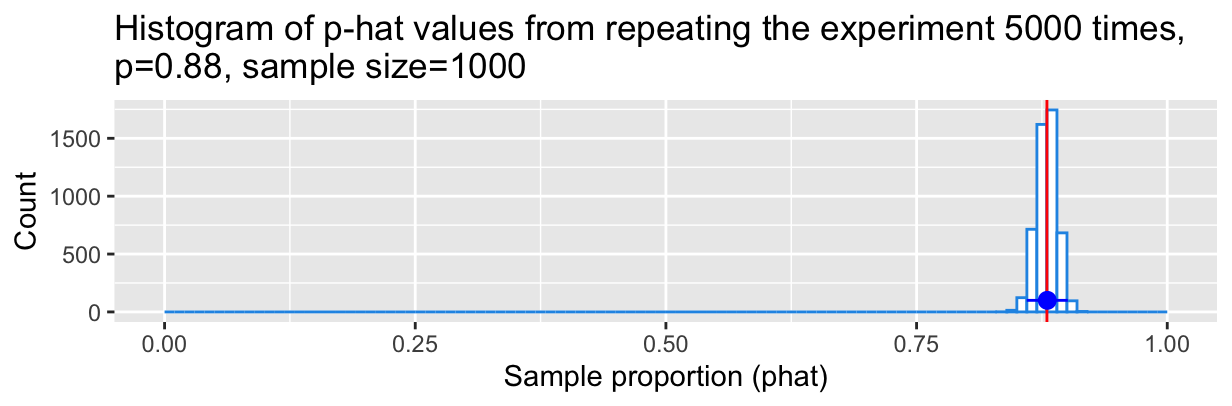
\includegraphics[width=0.75\textwidth]{sampling_distribution.png}
%     \end{center}
    
%     \soln{
%     \begin{table}[h!]
%         \centering
%         \begin{tabular}{|c|c|c|c|}
%         \hline
%          & Middle? & Symm? & Wider/Narrower/Same? \\ 
%         \hline
%         p=0.88, n=1000 & $\sim0.88$ & Yes & Same \\ 
%         \hline
%         p=0.5, n=100 & $\sim0.5$ & Yes & Wider \\ 
%         \hline
%         p=0.99, n=100 & $\sim0.99$ & No & Same? \\ 
%         \hline
%         \end{tabular}
%     \end{table}
%     }
% \end{frame}

% \begin{frame}
%     \frametitle{Edfinity Quiz}
%     What would happen if the sample size were 10?
% \end{frame}

% %%%%%%%%%%%%%%%%%%%%%%%%%%%%%%%%%%

% \section{R Demo: What would happen if...}

% %%%%%%%%%%%%%%%%%%%%%%%%%%%%%%%%

% \section{Board work: Deriving theoretical sampling distribution of the sample proportion}

% \begin{frame}
% \frametitle{Summary: theoretical sampling distribution of the sample proportion}
% \begin{itemize}
%     \item For a sample of size $n$ and population proportion $p$, the number of successes $X \sim \text{Binomial}(n, p)$
%     \item The sample proportion is a rescaled version of $X$: $\hat{p} = \frac{X}{n}$
%     \pause
%     \item So the sampling distribution of $\hat{p}$ is just like the binomial distribution, but for values from $0$ to $1$ instead of $0$ to $n$
%     \pause
%     \item $Pr(\hat{p} = \frac{k}{n}) = Pr(X = k) = \dbinom{n}{k} p^k (1-p)^{n-k}$ for $\frac{k}{n}$ in $\left\{0, \frac{1}{n}, \frac{2}{n}, \ldots, \frac{n-1}{n}, 1\right\}$
%     \pause
%     \item $E[\hat{p}] = p$
%     \item $Var[\hat{p}] = \frac{p(1-p)}{n}$
% \end{itemize}
% The \hl{Standard Error} is the standard deviation of the sampling distribution. Here, $SE_{\hat{p}} = \sqrt{\frac{p(1-p)}{n}}$
% \end{frame}
% %%%%%%%%%%%%%%%%%%%%%%%%%%%%%%%%%%

% \begin{frame}
%     \frametitle{Rule of succession}

%     There can be multiple statistics that estimate the same population parameter
%     \begin{itemize}

%         \item \hl{The Rule Of Succession} (Laplace, 18th Century)
%         \item What is the probability that the sun will rise tomorrow, given that it has risen every day for the last 5000 years?
%         \item 0 is an unsatisfying answer
%         \item Approach: Pretend we have seen one success and one failure
    
%     \end{itemize}

%     Sample proportion:
%      \begin{align}
%         \hat{p}=\frac{k}{n}
%     \end{align}
 
%     Rule of Succession:
%     \begin{align}
%         \hat{p}^*=\frac{k +1}{n+2}
%     \end{align}
 
% \end{frame}


% %%%%%%%%%%%%%%%%%%%%%%%%%%%%%%%%%%%%

% \section{R Demo: Comparing different estimators based on their sampling distributions}

% %%%%%%%%%%%%%%%%%%%%%%%%%%%%%%%%%%
% \begin{frame}
%     \frametitle{Comparing different estimators based on their sampling distributions}

%     \begin{itemize}
%         \item We can use simulations to compare different estimators for the same population parameter
%         \item In general, we want an estimator that
%         \begin{itemize}
%             \item is unbiased, i.e. the mean of the sampling distribution is equal to the population parameter
%             \item has low variability, i.e. the standard error is small
%         \end{itemize}
%         \item Often, there is a trade-off between bias and variability
%     \end{itemize}
% \end{frame}

%%%%%%%%%%%%%%%%%%%%%%%%%%%%%%%%
% End document
%%%%%%%%%%%%%%%%%%%%%%%%%%%%%%%%%%%%

\end{document}